\documentclass[a4paper,11pt, oneside]{book}
\usepackage[utf8]{inputenc}
\usepackage[francais]{babel}
\usepackage[T1]{fontenc}
\usepackage{graphicx}
\usepackage{float}
\usepackage{wrapfig}
\usepackage{setspace}
\usepackage{geometry}
\usepackage{hyperref}
\usepackage{multicol}
\usepackage{etoolbox}
\usepackage{color}
\usepackage[explicit,pagestyles]{titlesec}
\usepackage[absolute,overlay]{textpos}
\usepackage{fancyhdr}
\usepackage{fontspec}
\usepackage{eurosym}
\usepackage{titlesec}
\usepackage[]{algorithm2e}


% ====== CONFIG ========

%\setmainfont{Roboto Light}

%\setmainfont{Roboto Light}
%\setsansfont{Roboto}
%\setmonofont{Roboto}
%\newfontfamily\light{Roboto Slab Light}
\graphicspath{{img/}}
\setlength{\unitlength}{1mm}
\makeatletter

\definecolor{primary}{RGB}{44, 62, 80}


\titleformat{\chapter}[display]{\huge}{\thechapter \quad #1}{0pt}{}
\titlespacing{\chapter}{0pt}{0pt}{0pt}

\titleformat{\section}[display]{\LARGE}{}{0pt}{\thesection \quad #1}


\setlength{\TPHorizModule}{1mm}
\setlength{\TPVertModule}{1mm}
\def\sizeMedia{38}
\def\size{3.8cm}
\def\sizeMargin{0.2cm}
\def\margin{2}
\def\fixMargin{0}

\pagestyle{plain}

\author{Yann Prono, Quentin Tardivon}
\date{\today}

\def\school{TELECOM Nancy}
\def\schoolAddress{193 Avenue Paul Muller}
\def\schoolPostalCode{54602}
\def\schoolCity{Villers-lès-Nancy}
\def\schoolCodeAndCity{\schoolPostalCode, \schoolCity}
\def\schoolYear{2016 - 2017}

\def\appName{MyAdblock}
\def\widthImage{1}
\def\todo{{\color{red}\Huge{TODO}}}

\def\schoolYear{2016 - 2017}

% ====== END CONFIG ========


\begin{document}

	\begin{titlepage}
		\thispagestyle{empty}

{\color{primary}



\includegraphics[width=4.0cm]{img/school-logo.eps}
\hspace{9mm}

\includegraphics[width=4.0cm]{img/collegium-logo.eps}
\hspace{5mm}

\includegraphics[width=4.0cm]{img/university-logo.eps}

\vspace{0.5cm}

	\begin{center}


			{\color[rgb]{0.8,0.8,.8}\rule{\textwidth}{0.8pt}}
			\vspace{0.5cm}

			\baselineskip=3pt
			{\Huge \bfseries{\appName}}\\
			\vspace{0.2cm}
			{\huge \bfseries{Réseaux et systèmes avancées}}
			\vspace{0.5cm}

		{\color[rgb]{0.8,0.8,.8}\rule{\textwidth}{0.8pt}}
		\vspace{0.5cm}


		
\includegraphics[width=0.6\textwidth]{logo.png}

		\Large{Quentin Tardivon}\\
		\Large{Yann Prono}

		\vspace{1.5cm}
		\large{\schoolYear}
	\end{center}

}

	\end{titlepage}


	\newpage\newpage\null\thispagestyle{empty}
	\newpage
		\tableofcontents
		\thispagestyle{empty}


	\chapter{Introduction}
	\setcounter{page}{1}

		La publicité sur internet est un moyen simple de gagner de l'argent.
		Celles-ci sont intégrés au sein même du site web (vidéos, bannières publicitaires...). L'abondance de contenus publicitaires apportent
		cependant quelques désavantages: L'utilisateur peut être distrait par ces publicités, la lecture du site web est plus difficile
		étant donnée la quantité d'information et l'affichage de ces publicités demandent plus de bande passante
		ainsi que de ressources pour le navigateur web. Il existe cependant des logiciels permettant de supprimer
		ces publicités. Ces logiciels vont analyser le flux entrant et sortant du navigateur afin de filtrer le contenu publicitaire.\\

		\noindent Dans le cadre de ce projet, nous devons développer un proxy ayant la même fonctionnaalité qu'un bloqueur de publicités.
		Ce proxy sera programmé en langage C à l'aide des sockets vus durant les cours.


	\chapter{Analyse}

		Afin de comprendre comment il est possible de filtrer les publicités, il est nécessaire de comprendre fonctionne un navigateur web.
		On dispose de :
		\begin{itemize}
			\item Un navigateur web (le choix a peu d'importance dans le cadre de ce projet)
			\item Wireshark, un logiciel permettant capturer les paquets entrants et sortants de la machine\\
		\end{itemize}
		\noindent L'analyse des échanges TCP et HTTP se feront sur le site
		\href{http://www.telecomnancy.univ-lorraine.fr}{http://www.telecomnancy.univ-lorraine.fr}.
		Le site \href{http://www.01net.com}{http://www.01net.com} quant à lui sera utilisé pour
		analyser et tester le filtrage de publicités (abondance de publicités et la communication avec ce site n'est pas chiffrée).


		\section{Analyse du site telecomnancy.univ-lorraine.fr}

		Lorsque l'on souhaite accéder au site \href{http://www.telecomnancy.univ-lorraine.fr}{http://www.telecomnancy.univ-lorraine.fr} (on suppose que l'on dispose de l'adresse
		IP du serveur), des requêtes TCP (12, 13 et 14) sont envoyés au serveur afin d'initialiser la phase de connexion
		Suite à cela, une requête HTTP (15) de type \textit{GET} est envoyée au serveur afin de le contenu HTML du site web. La réponse du serveur est
		obtenue au paquet 29. Le contenu HTML est alors affiché dans le navigateur:

		\begin{figure} [htbp]
			\centering
			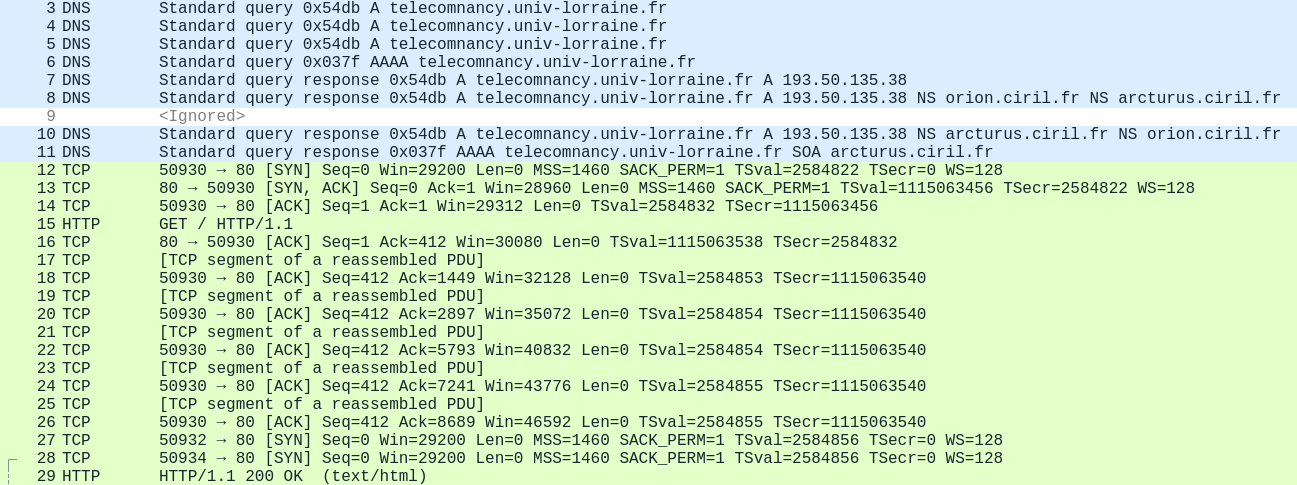
\includegraphics[width=\widthImage\textwidth]{1.png}\\
			\caption{Echanges de paquets au début de la communication}
		\end{figure}

		\noindent Cependant, le contenu HTML dépend d'autres ressources. Il est donc nécessaire
		récupérer les différentes ressources (images, fichiers CSS, fichiers JS). De nouvelles requêtes sont alors envoyées (35, 38, 41...):

		\begin{figure} [htbp]
			\centering
			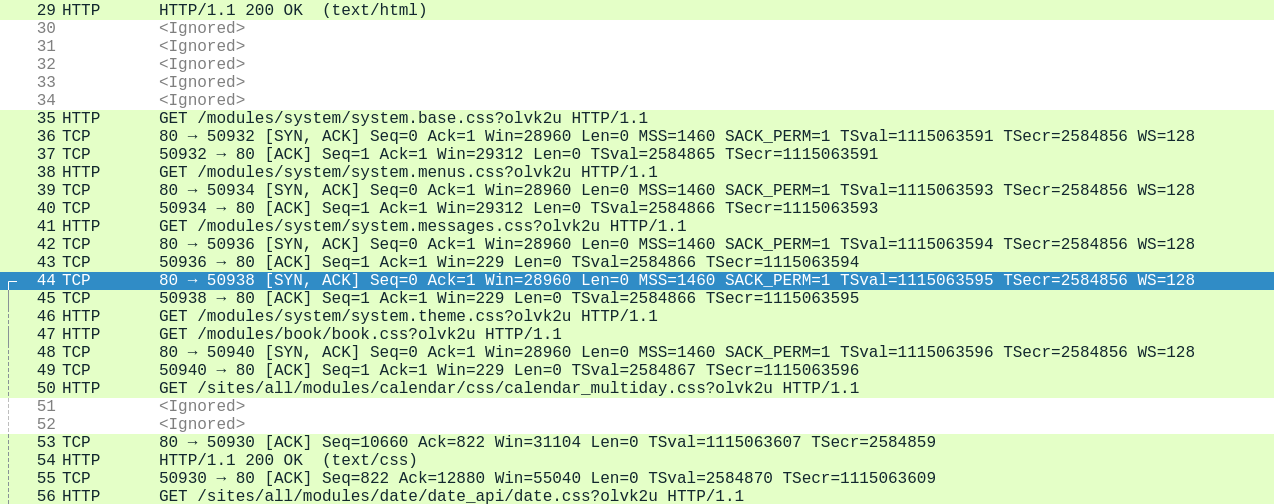
\includegraphics[width=\widthImage\textwidth]{2.png}\\
			\caption{Nouvelles requêtes émises suite à la réception du contenu HTML}
		\end{figure}

		On peut également retrouver l'ensemble de ces requêtes dans l'outil de développement intégré dans les navigateurs web:

		\begin{figure} [htbp]
			\centering
			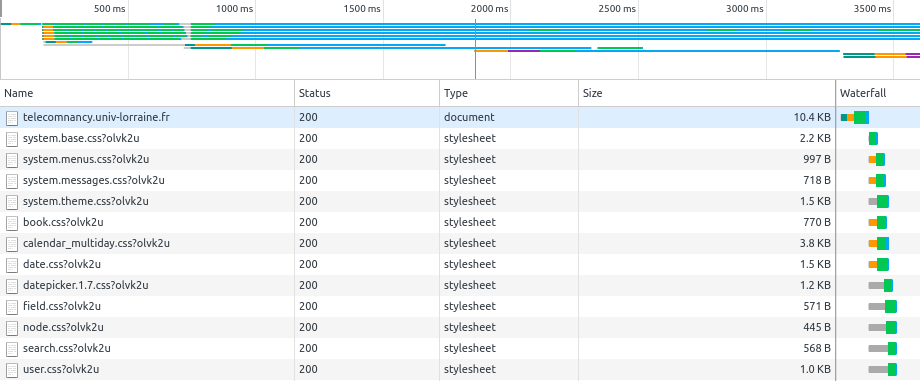
\includegraphics[width=\widthImage\textwidth]{3.png}\\
			\caption{Requêtes HTTP effectuées par le navigateur web}
		\end{figure}


	\clearpage
	\section{Analyse du site 01net.com}
		Le site contient de nombreux contenus publicitaires. Voici quelques requêtes permettant
		de faire une hypothèse sur l'algorithme à développer:

		\begin{figure} [htbp]
			\centering
			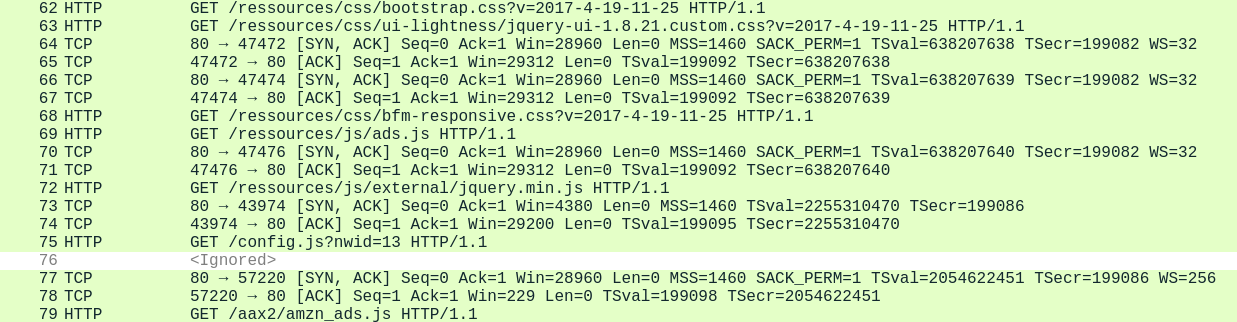
\includegraphics[width=\widthImage\textwidth]{4.png}\\
			\caption{Requêtes HTTP pour la demande de publicités}
		\end{figure}

		Des requêtes sont faites afin de demander des ressources utiles au bon fonctionnement du site (62 pour le style avec Bootstrap twitter, 63 pour JQuery).
		D'autres sont faites afin de charger les publicités sur le site: requête 69, 75 et 79.
		Si on s'intéresse à ces trois requêtes précédentes, on peut remarquer plusieurs caractéristiques:
		\begin{itemize}
			\item Les requêtes peuvent faire appel à une ressource directement chez un service tiers: pour la requête 79,
			on a dans la requête HTTP le champ  \textit{Host: c.amazon-adsystem.com}.
			\item la réponse à une requête peut rediriger vers une autre URL disponible sur un autre serveur:
			on a dans la réponse HTTP de la requête 75 le champ \textit{Location: http://ak-ns.sascdn.com/diff/js/smart.js}, cela
			signifie que le navigateur devra faire une nouvelle requête à l'adresse indique dans le champ \textit{Location}.
			\item \todo depend de ce que tu utilises quentin lors du filtrage
		\end{itemize}

		\clearpage
		On peut donc en déduire l'algorithme à utiliser afin de bloquer les publicités:\\

		\begin{algorithm}[H]
			\KwData{
				\begin{itemize}
					\item req: Requête du navigateur web à traiter
					\item blacklist: Liste des URL à rejeter
				\end{itemize}
			}
			\eIf{req.Host appartient à blacklist}{
				Rejeter la requête;\\
				Signaler le navigateur web du rejet de la requête;
   		}
			{
				Envoyer la requête au serveur;\\
				Attendre la réponse;\\
				Envoyer la réponse au navigateur web;
			}
		\end{algorithm}


		\chapter{Développement}

			Afin de réaliser \appName, nous nous sommes fortement inspirés du schéma présent sur le sujet.
			Notre proxy dispose de trois parties:
			\begin{itemize}
				\item La socket \textbf{server}
				\item La socket \textbf{dialog}
				\item La socket \textbf{client}
			\end{itemize}

			Chaque partie est détaillée dans la suite de ce document.


		\section{Socket server}

			La socket \textbf{server} est le point d'entrée du proxy. Au lancement du programme \appName,
			il sera nécessaire de configurer le navigateur web afin qu'il utilise comme proxy le serveur du programme.
			Dans le cadre de notre projet, le serveur fonctionne en local sur la machine. L'adresse IP est donc \textit{127.0.0.1}. Le port
			à utiliser peut être précisé par l'utilisateur, sinon le programme choisit un port disponible.

			Cette partie du programme est représentée par le fichier \textbf{server.c}. La structure \textit{server} réunit toutes les informations
			afin d'initialiser la socket. Après l'appel des fonctions bind() et listen, il est nécéssaire
			d'appeler \textit{accept\_server(...)}. Cette fonction accepte toute communication se connectant sur le serveur
			et initialise la socket de dialogue afin de traiter la requête HTTP. Le multi-clients a été géré à l'aide d'un fork. \todo formulation chelou


		\section{Socket dialog}

			La socket \textbf{dialog} est utilisée afin de communiquer entre le navigateur web et le proxy. Cette socket est créée
			suite à la méthode \textit{accept()} sur la socket du serveur. Cette socket est représentée par le fichier \textbf{dialog.c}.
			La version de notre programme traite uniquement les requêtes de type \textit{GET} en HTTP. Cette vérification s'effectue au niveau de la socket
			de dialogue. Si les conditions sont vérifiées, alors une socket client est initialisée afin de communiquer avec le serveur HTTP ciblé.

		\section{Socket client}

			La socket \textbf{client} permet de communiquer avec un serveur web. Le client va se connecter au serveur ciblé grâce à son adresse IP
			et envoyer la requête HTTP du navigateur web. La réponse est ensuite renvoyée
			au client qui lui la transmettras à la socket de dialogue.
			\todo
			On va créer une nouvelle requête HTTP à partir de celle reçu par le navigateur et l'envoyer directement au serveur web.
			C'est cette partie du programme qui se charge de la traduction des adresses pour la création du socket.

		\section{Adfilter}

			Lors de la création de la socket de dialogue, on va réaliser le filtrage des adresses émises par les requêtes GET.
			On initialise un tableau contenant la totalité des adresses présentes dans le fichier easylist. On va ensuite comparer l'adresse de
			la requête avec les entrées du tableau. Si jamais l'adresse correspond à une entrée, on ne communique pas la requête au socket client.

		\section{Problèmes rencontrées}

			Au cours du développement, nous avons rencontrées plusieurs difficultés.
			Premièrement, l'utilisation du langage C a été un frein important notamment pour tout ce qui est
			manipulation de chaînes de caractère.
			Le filtrage des publicités repose principalement sur la recherche de chaînes de caractères dans le header HTTP des requêtes.\\
			Utiliser le langage C pour ce genre de programmation devient fastidieux et instable.

			\noindent Nous avons rencontrés des difficultés au tout début du développement.
			La première version du programme devait simplement transmettre les requêtes au serveur ciblé sans aucun filtre.
			Cependant, le proxy ne fonctionnait pas sur certains sites notamment \href{http://www.01net.com}{www.01net.com}.
			En analysant les headers HTTP émises par le navigateur web, nous avons porté attention sur le champ
			\textit{Connection: keep-alive}. Cette valeur signifie que le navigateur doit garder ouvert la connection (la socket) ouverte
			pour les futures requêtes. Or dans le cas de notre proxy, si une socket traite une requête donnée, elle ne peut
			pas traiter les autres requêtes qui arrivent en même temps. Par conséquent, celles arrivant durant le traitement sont perdus par
			le proxy. Afin de contourner ce problème,
			nous avons décidé de réécrire le header HTTP pour chaque requête. Cette réécriture
			modifie uniquement la valeur du champ \textit{Connection} en le mettant à la valeur \textit{close}.
			Cette valeur à pour effet de fermer la connection lorsque la réponse est envoyée au navigateur. Cela permet
			également de créer une socket pour chaque requête faite par le navigateur, évitant de perdre des requêtes HTTP.
			Nous avons mis en place la recherche dans le fichier easylist, mais aucun des domaines présent ne fait partie du fichier.
			En effet, notre proxy ne laisse pas passer les requêtes \it{CONNECT} dans lesquels nous avons remarquer que certaines addresses étaient
			présentes dans le fichier easylist.

		\section{Améliorations possibles}

			Il aurait été possible d'apporter des améliorations à notre programme, afin d'en améliorer son efficacité en terme
			de nombre de pub bloqué. En effet, on remarque dans easylist plusieurs sections et nous n'exploitons que la première partie
			de ce fichier. On pourrait penser à un bloqueur de pub plus complet, masquant les zones des fichiers HTML où apparaissent certaines
			pub intégré à la page. Cette partie n'a pas été réalisé car nous considérions qu'elle était peu pertinente dans le cadre du projet.
			Il aurait fallu au sein de notre serveur proxy, analyser le DOM et modifier les parties ayant une correspondance dans le fichier
			easylist.

			\chapter{Conclusion}

			 Nous avons vu la réalisation d'un proxy complet HTTP utilisant les socket système en C dans le but de réaliser un adblocker.
			 Nous avons donc suivi un raisonnement complet, de l'analyse de trace réseau à l'aide de Wireshark, jusqu'à l'implémentation
			 du proxy et du système de filtrage des pubs. 


			\chapter{Bibliographie}
			\begin{itemize}
				\item \textit{Hypertext Transfer Protocol}, Wikipedia, \\\href{https://en.wikipedia.org/wiki/Hypertext\_Transfer\_Protocol}
				{wikipedia.org/wiki/Hypertext\_Transfer\_Protocol}, consulté le 20 avril 2017

				\item \textit{HTTP persistent connection}, Wikipedia, \\\href{https://en.wikipedia.org/wiki/HTTP\_persistent\_connection}
				{wikipedia.org/wiki/HTTP\_persistent\_connection}, consulté le 15 avril 2017

				\item \textit{Créer des filtres Adblock Plus}, Adblock Plus, \href{https://adblockplus.org/fr/filters}{adblockplus.org/fr/filters}, consulté le 16 avril 2017
				\item easylist, \href{https://easylist.to/}{easylist.to}, consulté le 10 avril 2017
			\end{itemize}


\end{document}
